\documentclass[aps,pre,twocolumn,superscriptaddress,nofootinbib,floatfix]{revtex4-2}
\usepackage{amsmath,amssymb,amsthm}
\usepackage{graphicx}
\usepackage{booktabs}
\usepackage{bm}
\usepackage[colorlinks=true,linkcolor=blue,citecolor=blue,urlcolor=blue]{hyperref}

\newtheorem{theorem}{Theorem}
\newtheorem{lemma}{Lemma}
\newtheorem{conjecture}{Conjecture}
\newcommand{\AD}{\mathrm{AD}}
\newcommand{\Bin}{\mathrm{Bin}}
\newcommand{\dd}{\mathrm{d}}

\begin{document}

\title{Electrostatics of forced defects in dimer coverings:\\ corner charges, image charges, and boundary chemical potentials}

\author{Changyeon Won}
\email{cywon@khu.ac.kr}
\affiliation{Department of Physics, Kyung Hee University, Seoul 02447, Republic of Korea}

\date{\today}

\begin{abstract}
When a planar region cannot be covered completely by dimers, for example because two diagonally opposite corners of a chessboard have been removed, the uncovered sites (monomers) are forced to appear somewhere. We ask where they sit when all admissible configurations are equally likely. We answer this question with exact enumeration, using transfer matrices and Kasteleyn determinants for boards up to $512$ sites across, and interpret the result physically. The forces acting on the defects are purely entropic, yet the defects behave as charges of a two-dimensional Coulomb gas. The close-packing constraint acts as a lattice Gauss law, and the dimer height field plays the role of the electrostatic potential. For boundaries parallel to the lattice axes, every corner carries a fractional charge $q_c=-J_c/4$, where $J_c$ is the jump of the boundary height at the corner ($\pm1/4$ for an ordinary corner and $+3/4$ for a removed one). A free boundary acts as a mirror that produces image charges of the \emph{same} sign. With these rules, a conformally covariant density formula reproduces the exact defect distributions in all rectangles with no adjustable parameter, to 1--3\% accuracy. We derive the corner-to-boundary law $4/[\pi(x+1)]$ exactly. We show that all string determinants reduce to Toeplitz(+Hankel) determinants of a single scalar symbol, $\sigma(\varphi)=\mathrm{sgn}(\cos\varphi)(\cos\varphi+i)/\sqrt{1+\cos^2\varphi}$. We identify the amplitudes of the bulk, half-plane and quadrant correlations as $\pi2^{-3/4}G(\tfrac12)^4$, $2^{3/8}G(\tfrac12)^2$ and $2^{9/8}G(\tfrac12)^2$ ($G$ is the Barnes function). Staircase boundaries behave qualitatively differently: in the Aztec diamond the defects are trapped in a boundary layer where the arctic circle touches the edge. We explain this crossover with a boundary chemical potential $\mu=\delta\ln Z/\delta h_{\partial}$. We compute $\mu$ from the limit shape by continuing the complex Burgers solution along tangent lines into the frozen region, and it reproduces the exact large-deviation law of the Aztec diamond identically. It also predicts, without free parameters, the exponential trapping rate in mixed straight/staircase domains. When the defect path crosses frozen boundaries, an additional layer-removal cost $\partial\ln Z/\partial(\text{size})$ and a competition between nested channels appear. This rule, inferred from the Aztec diamond, is confirmed independently on lozenge tilings of hexagons to within $0.5\%$.
\end{abstract}

\maketitle

%=====================================================================
\section{Introduction}
%=====================================================================

Close-packed dimers on a lattice are among the oldest exactly solvable problems of statistical mechanics~\cite{Kasteleyn1961,TemperleyFisher1961,FisherStephenson1963}. They also serve as a paradigm for the physics of local constraints. The constraint that every site is covered exactly once turns the dimer configurations into a divergence-free flux. It endows the model with a height field that is critical and Gaussian at long wavelengths~\cite{Kenyon2000,Kenyon2001,Nienhuis1984,Henley2010}. It also turns monomers (uncovered sites) into topological defects: vortices of the height field, or charges of an emergent electrostatics. The same ``Coulomb phase'' physics appears in three-dimensional dimer models~\cite{Huse2003}, in spin ice, where violations of the ice rule behave as magnetic monopoles~\cite{Castelnovo2008}, and in artificial spin-ice arrays where such defects can be imaged directly~\cite{Wang2006,Ladak2010}. In all these systems the effective interaction between defects is, at least in part, \emph{entropic}. No energy is involved; defects attract or repel only because their positions change the number of available configurations.

Most of what is known about monomers concerns pairs in the bulk~\cite{FisherStephenson1963,Hartwig1966,FendleyMoessnerSondhi2002}, pairs on a straight boundary~\cite{PriezzhevRuelle2008}, holes of prescribed charge in lozenge tilings~\cite{Ciucu2010,CiucuKrattenthaler2011}, or monomers pinned at corners~\cite{Allegra2015}. Here we consider a different and very elementary question. Suppose a finite region is unbalanced, so that it \emph{cannot} be tiled completely. The classic example is the ``mutilated chessboard'' with two opposite corners removed. Then defects are forced to exist. If every admissible configuration is equally likely, where are the defects?

The question is natural from a physical point of view. The defects are free to move, but the boundary of the region interacts with them through the entropy of the dimer sea. Their distribution is therefore a direct, parameter-free probe of how a boundary couples to the emergent electrostatics. We find two qualitatively different regimes, and a single framework that connects them.

(i) For boundaries parallel to the lattice axes (chessboard-like regions, Figs.~\ref{fig:schematic}--\ref{fig:odd}), the defects behave as charges of a two-dimensional Coulomb gas in the presence of fractional \emph{corner charges} $q_c=-J_c/4$ and \emph{same-sign images} at free boundaries. A conformally covariant density formula, Eq.~\eqref{eq:density}, then describes the exact distributions of single and paired defects in all rectangles, with no adjustable parameter. The amplitudes of the corresponding lattice correlations turn out to be simple Barnes-$G$ expressions (Sec.~\ref{sec:exact}).

(ii) For staircase (diagonal) boundaries, exemplified by the Aztec diamond, the region contains frozen corners separated from a liquid region by an arctic circle~\cite{JockuschProppShor1998}. There the defects are not governed by power laws. Instead they are trapped \emph{exponentially} in a boundary layer near the points where the arctic circle touches the boundary (Sec.~\ref{sec:aztec}).

The two regimes are unified by a \emph{boundary chemical potential} $\mu(s)=\delta\ln Z/\delta h_\partial(s)$ (Sec.~\ref{sec:mu}). This is the response of the macroscopic entropy to a shift of the boundary height, which is precisely the perturbation created by a defect and its ``string''. On a flat, liquid-adjacent boundary $\mu=0$, and only the Coulomb-gas power laws survive. On frozen or tilted boundaries $\mu\neq0$ and the defect weight acquires a factor $\exp(\int\mu\,\dd s)$. We show how to compute $\mu$ from the limit shape of Cohn, Kenyon, Okounkov, and Propp~\cite{CohnKenyonPropp2001,KenyonOkounkov2007}. The result reproduces the exact Aztec-diamond law identically and predicts trapping rates in mixed domains. We also identify when this linear response must be supplemented by a geometric ``layer'' term and a competition between channels, and we test the resulting rule on a different lattice.

Throughout we distinguish carefully between rigorous results, results established by exact arithmetic to many digits, numerically supported statements, and conjectures. A summary is given in Table~\ref{tab:summary}.

%---------------------------------------------------------------------
\begin{figure*}[t]
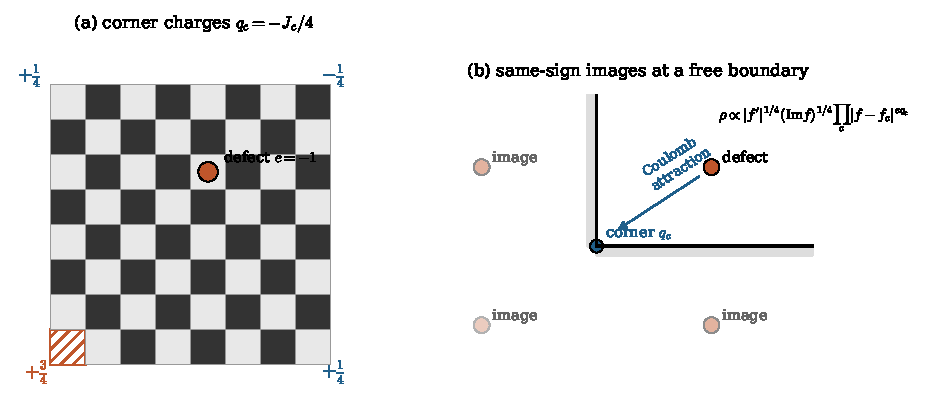
\includegraphics[width=0.85\textwidth]{figs/fig1_schematic.pdf}
\caption{(a) An $8\times8$ board with corner a1 removed. The region has one more white than black square, so one white defect (charge $e=-1$) is forced. Each corner carries the fractional charge $q_c=-J_c/4$ given by the jump $J_c$ of the boundary height: $-1/4$ for a black corner, $+1/4$ for a white corner and $+3/4$ for the removed black corner. (b) In the continuum description a free edge acts as a mirror with images of the same sign, and the corners act as fixed charges. The resulting density of a single defect is given by Eq.~\eqref{eq:density}.}
\label{fig:schematic}
\end{figure*}

%=====================================================================
\section{Model and methods}
\label{sec:model}
%=====================================================================

\subsection{Dimers, heights and charges}
We consider unions of unit squares (cells) of $\mathbb{Z}^2$, colored like a chessboard; cell $(x,y)$ is black if $x+y$ is even. A domino covers one black and one white cell. If the region has $n_w$ white and $n_b$ black cells, at least $|n_w-n_b|$ cells remain uncovered. We study the uniform measure on configurations with exactly the forced number of defects. We call the white defects negative ($e=-1$) and the black defects positive ($e=+1$). A removed cell carries the charge of a defect of its color.

The Thurston height $h_T$ changes by $+1$ ($-1$) when one walks along a lattice edge with a black (white) cell on the left. Around a covered vertex $h_T$ returns to its value. Around a defect it winds by $\pm4$, so the defect is a vortex of the height field. We use the normalized height $h=h_T/2$, whose admissible slopes satisfy $|h_x|+|h_y|\le1$. In the scaling limit $h$ converges to a Gaussian free field~\cite{Kenyon2000,Kenyon2001}, and defects become electric charges of the dual (magnetic) description~\cite{Nienhuis1984,Henley2010}.

\subsection{Exact enumeration}
We use three independent exact methods.
(a) A row-by-row broken-profile transfer matrix with 128-bit integers, which gives exact counts for all defect configurations on boards up to $N=16$. It serves as the reference.
(b) Kasteleyn determinants~\cite{Kasteleyn1961}, with horizontal weights $1$ and vertical weights $i$ (or real signs alternating by column). For regions with interior defects, the Kasteleyn condition is restored by flipping the signs of the edges crossed by a ``string'' joining the defect to the boundary.
(c) A low-rank update. If $G=K^{-1}$ is known for the defect-free region, the ratio of partition functions with defects at $v$ and $c$ is the bordered determinant
\begin{equation}
\frac{Z(\Omega\setminus\{c,v\})}{Z(\Omega)}=\left|\det\begin{pmatrix}I-2G(b_j,w_l) & -2G(b_j,v)\\ G(c,w_l) & G(c,v)\end{pmatrix}\right|,
\label{eq:bordered}
\end{equation}
where $(b_j,w_l)$ are the endpoints of the string edges.
For the infinite plane, half plane and quadrant, the entries of $G$ are exact numbers of the form $a+b/\pi$ with rational $a,b$. We generate them by an exact recursion and evaluate determinants in ball arithmetic (Arb) with certified error bounds, up to string lengths $r=1024$.
On $8\times8$ boards the three methods agree for all 1552 defect configurations. Aztec-diamond ratios were obtained from exact integer inverses (FLINT), because double precision fails beyond $n\simeq44$ (the condition number reaches $\sim10^{17}$ at $n=64$).
All key claims of Secs.~\ref{sec:exact}--\ref{sec:mu} were independently re-derived from scratch by a separate code base; no discrepancy was found.

%=====================================================================
\section{Coulomb gas for axis-parallel boundaries}
\label{sec:coulomb}
%=====================================================================

\subsection{Corner charges from boundary height jumps}
Walking counterclockwise along the boundary, the height oscillates between two values on a straight edge, so its average is constant along each edge. At a convex corner the corner cell contributes two consecutive steps of the same sign. The average height therefore jumps by $J_c=+1$ at a black corner and $J_c=-1$ at a white corner. At the notch of a removed black corner four consecutive $-1$ steps give $J_c=-3$, which differs from $+1$ by one monomer's worth of winding.

A jump $J$ at a boundary point $c$ creates an average height $(J/\pi)\arg(z-c)$. Its harmonic conjugate is $(J/\pi)\ln|z-c|$. A bulk monomer creates $(2/\pi)\ln|z-z_0|$ in the same normalization. Because the dual field obeys Neumann conditions, a charge on the boundary overlaps with its own image. Matching $2q\cdot(2/\pi)=J/\pi$ gives
\begin{equation}
\begin{split}q_c&=-\frac{J_c}{4}:\\ q&=-\tfrac14\ \text{(black)},\ +\tfrac14\ \text{(white)},\ +\tfrac34\ \text{(removed)}.\end{split}
\label{eq:corner}
\end{equation}
This is a purely combinatorial statement. The same boundary-height jumps were identified by Allegra~\cite{Allegra2015} as boundary-condition-changing operators of dimension $J^2/32$ at the corners. That work used them to compute corner free energies and correlations of monomers placed \emph{at} corners. Here we use them for the distribution of \emph{freely moving} defects.

\subsection{Density formula and corner exponents}
Let $f$ map the region conformally onto the upper half plane, and let $f_c=f(c)$ be the images of the corners. Treating the defect as a charge $e$ in the field of the corner charges and of its images, we obtain
\begin{equation}
\rho(z)\propto|f'(z)|^{1/4}\,[\mathrm{Im}f(z)]^{1/4}\prod_c|f(z)-f_c|^{e\,q_c}.
\label{eq:density}
\end{equation}
For two defects there is an additional factor $\left(|f_1-f_2|\,|f_1-\bar f_2|\right)^{e_1e_2/2}$. The factor $|f'|^{1/4}(\mathrm{Im}f)^{1/4}$ is the one-point function of a charge of dimension $1/4$ in the presence of a same-sign image. Near a corner of interior angle $\theta$, Eq.~\eqref{eq:density} predicts $\rho\sim r^{\gamma}$ with
\begin{equation}
\gamma=\frac{\pi}{\theta}\Bigl(\frac12+e\,q_c\Bigr)-\frac14 .
\label{eq:gamma}
\end{equation}
For a white defect next to the removed corner a1 ($\theta=\pi/2$, $q_c=3/4$), this gives $\gamma=-3/4$. The defect density thus \emph{diverges} as $r^{-3/4}$ toward the removed corner (Fig.~\ref{fig:single}). The exact slopes $0.754$ ($N=64\to128$) and, on the mutilated board, $0.750$ agree with this prediction. The formula also holds for concave corners, to three decimal places.

\begin{figure*}[t]
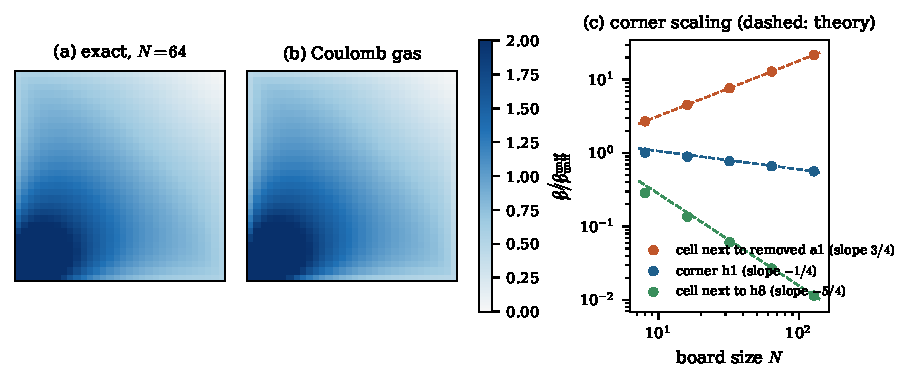
\includegraphics[width=\textwidth]{figs/fig2_single.pdf}
\caption{A single removed corner. (a) Exact defect density on a $64\times64$ board with a1 removed, averaged over $2\times2$ blocks and normalized to the uniform value. (b) The parameter-free Coulomb-gas prediction, Eq.~\eqref{eq:density}, computed with the Jacobi-elliptic map of the square. (c) Density at three special cells versus board size (exact, symbols), compared with the power laws predicted by Eq.~\eqref{eq:gamma} (dashed). The rms deviation between (a) and (b) is $0.9\%$ at $N=128$ and decreases as $1/N$. The orange square marks the removed cell a1.}
\label{fig:single}
\end{figure*}

\begin{figure*}[t]
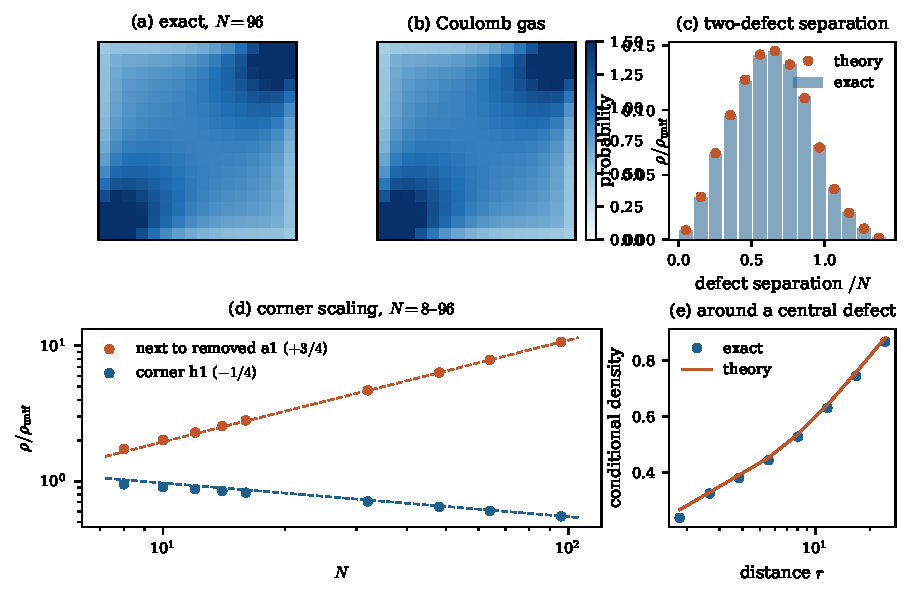
\includegraphics[width=\textwidth]{figs/fig3_mutilated.pdf}
\caption{The mutilated chessboard (corners a1 and h8 removed; two white defects). (a,b) Exact marginal density at $N=96$ ($2\times2$ block averages, each block containing exactly two white cells) compared with the two-defect Coulomb gas. Orange squares mark the removed corners a1 and h8. (c) Distribution of the defect separation. (d) Corner scaling for $N=8$--$96$; dashed lines show the slopes predicted by Eq.~\eqref{eq:gamma}. (e) Conditional density around a defect fixed at the centre. All theory curves are parameter free.}
\label{fig:mutilated}
\end{figure*}

\subsection{Tests}
We tested Eq.~\eqref{eq:density} on even$\times$even, odd$\times$odd and odd$\times$even rectangles, with corner, edge and interior cells removed, and with one or two defects (Figs.~\ref{fig:single}--\ref{fig:odd}). The rms deviations are 1--3\% at the largest sizes and decrease as $1/N$. Two special cases illustrate the physics.

\emph{Mutilated board} (Fig.~\ref{fig:mutilated}). The two defects are attracted by the two removed corners ($q=+3/4$ each) and repel each other. Their joint distribution, the corner scaling and the conditional density around a central defect all follow the Coulomb gas.

\emph{Odd$\times$odd board} (Fig.~\ref{fig:odd}). All four corners carry $q=+1/4$. For the black defect the total boundary charge is neutral, and Eq.~\eqref{eq:density} reduces to $\rho\propto R^{1/4}$, where $R$ is the conformal radius. The defect is pushed toward the centre, and the corner-to-centre ratio decays as $N^{-1/4}$. At the lattice level, the equal probability of all even-even boundary cells follows from Temperley's bijection. The defect lives on two black sublattices, (even,even) and (odd,odd), whose weights differ near the boundary (Fig.~\ref{fig:odd}a,b,d). This staggering is a lattice effect that the continuum formula averages over: the sublattice means differ by $0.42$, $0.27$, $0.17$ and $0.10$ (in units of $\rho_{\rm unif}$) for $N=7$, $15$, $31$ and $63$, and the average of neighbouring cells of the two sublattices follows $\rho\propto R^{1/4}$ to within $3\%$ everywhere except in the outermost row.

\begin{figure*}[t]
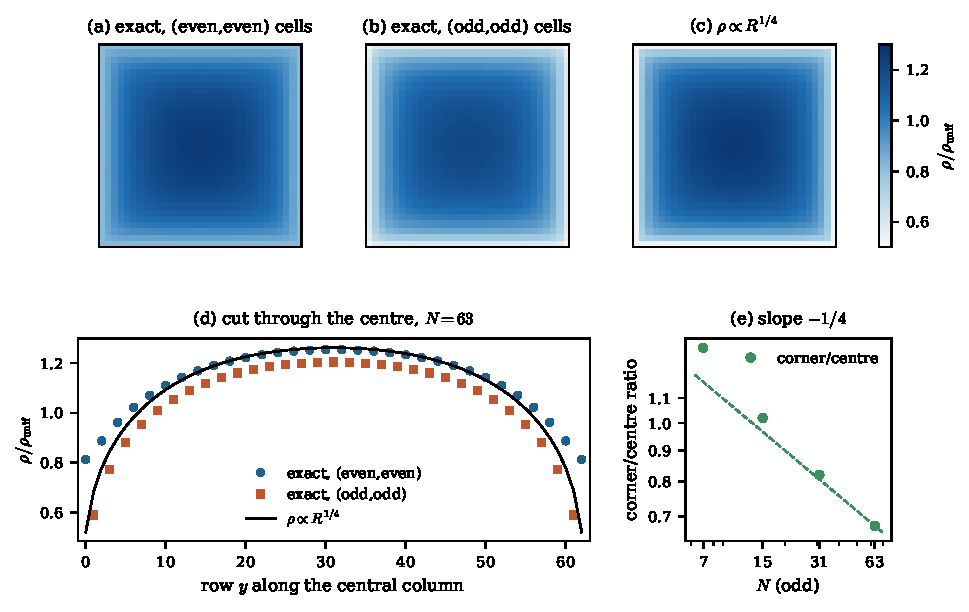
\includegraphics[width=\textwidth]{figs/fig4_odd.pdf}
\caption{Odd$\times$odd boards, where the boundary charge is neutral. (a,b) Exact defect density on a $63\times63$ board, shown cell by cell on the two black sublattices, (even,even) and (odd,odd), without averaging. (c) Prediction $\rho\propto R^{1/4}$, where $R$ is the conformal radius. (d) Cut along the central column: the two sublattices (symbols) bracket the prediction (line). (e) Corner-to-centre ratio versus $N$, with the predicted slope $-1/4$.}
\label{fig:odd}
\end{figure*}

\emph{Image charges.} A single defect near a straight free edge and a pair of defects confirm that the image has the \emph{same} sign as the source (Fig.~\ref{fig:pairs}a). The pair correlation decays as $d^{-1}$ along a boundary and as $d^{-1/2}$ in the bulk. The boundary-pair amplitude $2/(\pi d)$ agrees with the result of Priezzhev and Ruelle~\cite{PriezzhevRuelle2008}. At the lattice level the sign follows from the fact that the long-distance behaviour of $K^{-1}$ is dominated by momenta $\pm\pi/2$. A reflection that shifts by two lattice spacings then acquires a phase $e^{i\pi}=-1$, which converts the lattice Dirichlet reflection into a continuum Neumann (same-sign) image.

%=====================================================================
\section{Exact results and amplitudes}
\label{sec:exact}
%=====================================================================

\subsection{Corner to boundary}
\begin{theorem}[Quadrant, boundary defect]
In the infinite quadrant with its corner cell $c$ removed, place a white defect on the boundary cell $(x,0)$, with $x$ odd. Then, for $x\ge3$,
\begin{equation}
\begin{split}\frac{Z(Q\setminus\{c,(x,0)\})}{Z(Q)}&=\frac4\pi\int_0^{\pi/2}\!\sin\theta\,\sin[(x+1)\theta]\\&\qquad\times\sqrt{1+\cos^2\theta}\,\dd\theta\\
&=\frac{4}{\pi(x+1)}+O(x^{-3}).\end{split}
\label{eq:thmA}
\end{equation}
The values are of the form ``integer minus rational$/\pi$'', e.g.\ $2-16/(3\pi)$ at $x=3$.
\end{theorem}
The proof diagonalizes the box Kasteleyn matrix by sine functions and evaluates one integral in closed form. The leading term comes from $\theta=\pi/2$, and the next order vanishes by parity. The exponent $-1$ is the Coulomb-gas value $|f'|^{1/2}|f|^{-3/4}$ for $f=z^2$, while the prefactor $4/\pi$ is a lattice quantity.

\subsection{A single scalar symbol}
For a vertical string, the horizontal offset between the black end of the $j$th string edge and the white end of the $l$th depends only on the parity of $j-l$. Hence $I-2G$ is a Toeplitz matrix in $j-l$. Summing the Fourier series in closed form gives the symbol
\begin{equation}
\sigma(e^{i\varphi})=\mathrm{sgn}(\cos\varphi)\,\frac{\cos\varphi+i}{\sqrt{1+\cos^2\varphi}},
\label{eq:sigma}
\end{equation}
which is a pure phase with jumps of $\pi$ at the massless points $\varphi=\pm\pi/2$ (Fig.~\ref{fig:pairs}b). Moreover, when the defect sits at the end of the string and the removed cell at its start, the border row of Eq.~\eqref{eq:bordered} equals $-\tfrac12$ times the first row. It can therefore be eliminated exactly. With $c_m$ the Fourier coefficients of $\sigma$,
\begin{align}
R_{\rm bulk}(r)&=\tfrac12\left|\det\left[c_{j-k-1}\right]_{j,k=0}^{r-1}\right|,\\
R_{\rm half}(r)&=\tfrac12\left|\det\left[c_{j-k-1}-c_{j+k+3}\right]_{j,k=0}^{r-1}\right|,
\label{eq:reductions}
\end{align}
for a pair at vertical distance $r$ in the plane, and for a boundary cell and a defect at height $r$ above it in the half plane. The Hankel part in the second line is the lattice image charge.

\subsection{Amplitudes}
The symbol $z\sigma$ is of Fisher--Hartwig type with $\beta_1=\beta_2=\tfrac12$ at $z=\pm i$. The Deift--Its--Krasovsky asymptotics~\cite{DeiftItsKrasovsky2011} then gives
\begin{equation}
R_{\rm bulk}(r)\simeq \pi\,2^{-3/4}\,G(\tfrac12)^4\,r^{-1/2}=0.2473718\ldots\,r^{-1/2}.
\end{equation}
The factors are $2^{-1/4}$ from $\sum_k kV_kV_{-k}=-\mathrm{artanh}(q^2)$ with $q=\sqrt2-1$, $2^{1/2}$ from $|z_1-z_2|^{2\beta_1\beta_2}$, and $[G(\tfrac32)G(\tfrac12)]^2$ from the two jumps. The same constant was obtained for diagonal separation by Hartwig~\cite{Hartwig1966} ($B/4$ with $B=0.98948729$). Our derivation shows that the axis and diagonal amplitudes coincide, and it expresses the constant in closed form. For the half plane and the quadrant we established the amplitudes by certified arithmetic up to $r=1024$ and extrapolation, to 18--19 digits (Fig.~\ref{fig:pairs}c):
\begin{equation}
C_{\rm half}=2^{3/8}G(\tfrac12)^2,\qquad C_{\rm quad}=2^{9/8}G(\tfrac12)^2 .
\end{equation}
The pattern ``lattice value $=$ operator normalization $\times$ continuum Coulomb-gas correlator'' accounts for all three. The transcendental factor $G(\tfrac12)^2$ belongs to each bulk monomer, while the boundary and corner normalizations involve only $\pi$ and powers of $2$. A proof for the half plane would require the asymptotics of a Toeplitz+Hankel determinant with a \emph{non-even} Fisher--Hartwig symbol $z^{-1}\sigma$ of winding $-1$. This lies just outside the existing theory~\cite{DeiftItsKrasovsky2011,BasorEhrhardt2017,GharakhlooIts2020}.

\begin{figure*}[t]
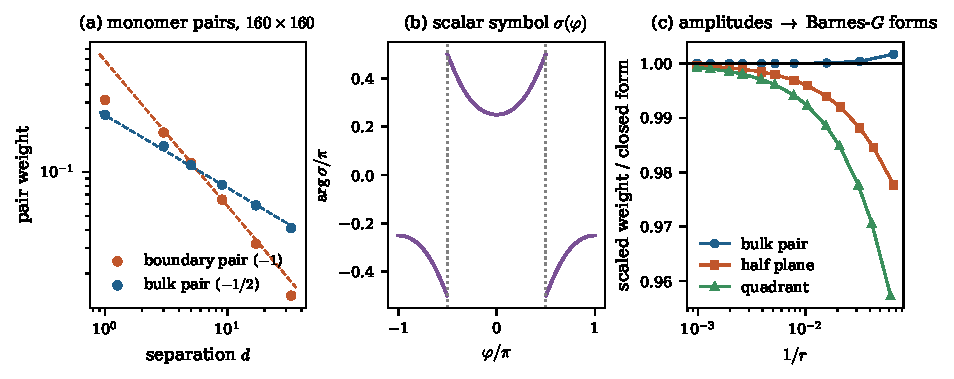
\includegraphics[width=\textwidth]{figs/fig5_pairs.pdf}
\caption{(a) Monomer-pair correlations on a $160\times160$ board: along the boundary ($\propto d^{-1}$, same-sign images) and in the bulk ($\propto d^{-1/2}$). (b) Phase of the scalar symbol $\sigma$ of Eq.~\eqref{eq:sigma}, with jumps of $\pi$ at $\varphi=\pm\pi/2$. (c) Exact weights, scaled by the expected power law and divided by the closed forms $\pi2^{-3/4}G(\tfrac12)^4$ (bulk), $2^{3/8}G(\tfrac12)^2$ (half plane) and $2^{9/8}G(\tfrac12)^2$ (quadrant), versus $1/r$.}
\label{fig:pairs}
\end{figure*}

%=====================================================================
\section{Staircase boundaries: trapping in the Aztec diamond}
\label{sec:aztec}
%=====================================================================

The Aztec diamond $\AD_n$ has $Z=2^{n(n+1)/2}$ tilings~\cite{EKLP1992}. Four frozen corners are separated from a liquid disk by the arctic circle~\cite{JockuschProppShor1998}. We remove the west tip cell $t$, which forces one white defect, and we also consider a missing domino, which forces two defects of opposite colours. In both cases the defects avoid the liquid region. Instead they stay within a boundary layer about two cells thick, near the points where the arctic circle touches the edges (Fig.~\ref{fig:aztec}a). The weight outside this layer decays as $n^{-1}$ for one defect and as $n^{-1/2}$ for a pair (Fig.~\ref{fig:aztec}c).

On the boundary the distributions are known exactly. Let $k$ be the position of the defect along the edge, counted from the tip. For the adjacent (SW) and the opposite (NE) edge,
\begin{align}
\frac{Z(\AD_n\setminus\{t,\mathrm{SW}_k\})}{Z(\AD_n)}&=P\bigl(\Bin(n,\tfrac12)\ge k\bigr),\label{eq:thmC}\\
\frac{Z(\AD_n\setminus\{t,\mathrm{NE}_k\})}{Z(\AD_n)}&=\binom{n-1}{k-1}2^{-n},\label{eq:thmD}
\end{align}
For a missing domino with defects at positions $k$ and $l$ on the two edges adjacent to a corner,
\begin{equation}
\begin{split}\frac{Z(\AD_n\setminus\{\mathrm{S1}_k,\mathrm{S2}_l\})}{Z(\AD_n)}=\sum_{j=0}^{n-1}2^{j-1}&\,P\bigl(\Bin(j,\tfrac12)=k-1\bigr)\\\times&\,P\bigl(\Bin(j,\tfrac12)=l-1\bigr).\end{split}
\label{eq:thmE}
\end{equation}
Equation~\eqref{eq:thmE} is equivalent to the boundary generating function of Chhita and Young~\cite{ChhitaYoung2014}, and Eqs.~\eqref{eq:thmC}--\eqref{eq:thmD} are special cases of it. We found these laws independently by exact computation. We also give elementary proofs of Eqs.~\eqref{eq:thmC} and \eqref{eq:thmD} that do not use urban renewal (Appendix~\ref{app:proofs}). Equation~\eqref{eq:thmE} has a transparent dynamical reading. In domino shuffling the defect pair is created at the corner at ``time'' $j$ with weight $\tfrac12$, and afterwards the two defects perform independent random walks along their edges. Summing the pair weights over all boundary positions gives $2^{n+1}-2=Z(\AD_{n+1})/Z(\AD_n)-2$.

\begin{figure*}[t]
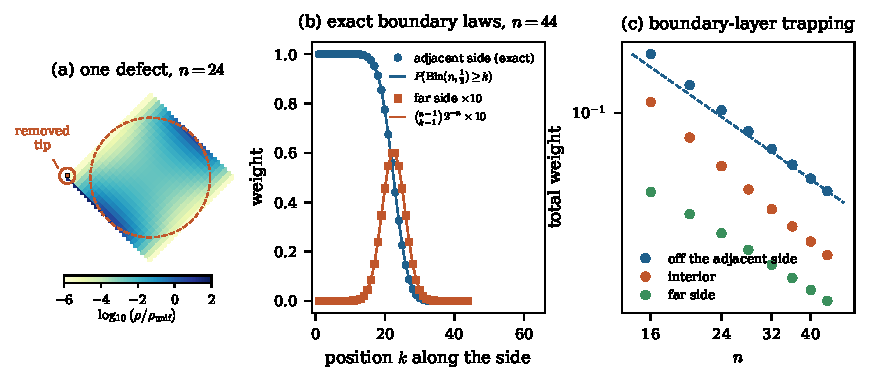
\includegraphics[width=\textwidth]{figs/fig6_aztec.pdf}
\caption{Aztec diamond with the west tip removed. (a) Exact defect density $\rho/\rho_{\rm unif}$ for $n=24$ on a logarithmic colour scale spanning eight decades; each cell of the defect sublattice is drawn as a diamond reaching its four neighbours. The dashed line is the arctic circle, and the small circle marks the removed tip. The density falls to $10^{-6}$ along the two edges that do not touch the removed tip and drops steeply near the far end of the adjacent edge, following the binomial tail of Eq.~\eqref{eq:thmC}. (b) Exact weights along the adjacent (south-west) and opposite edges for $n=44$ (symbols), compared with Eqs.~\eqref{eq:thmC}--\eqref{eq:thmD} (lines). (c) Total weight off the adjacent edge, in the interior and on the far edge, versus $n$.}
\label{fig:aztec}
\end{figure*}

%=====================================================================
\section{Boundary chemical potential}
\label{sec:mu}
%=====================================================================

\subsection{Definition}
A defect and the removed cell are joined, along the boundary, by an arc $\Gamma$ on which the boundary height is shifted by $\delta=2$ (one monomer of Thurston winding). To leading exponential order the defect weight is the change of the macroscopic entropy. For a small shift this is the linear response
\begin{equation}
\begin{split}\ln w&\simeq \delta\int_\Gamma\mu(s)\,\dd s,\\ \mu(s)&=\frac{\delta \ln Z}{\delta h_\partial(s)}=\mathbf n\cdot\nabla_{\!p}\,\mathrm{ent}(\nabla h)\big|_{\partial},\end{split}
\label{eq:mu}
\end{equation}
where $\mathrm{ent}$ is the Cohn--Kenyon--Propp local entropy~\cite{CohnKenyonPropp2001}, $h$ is the limit shape and $\mathbf n$ is the outward normal. On a flat, liquid-adjacent edge such as that of the chessboard, $\nabla h=0$ gives $\mu=0$. The exponential factor is then absent and only the Coulomb-gas power laws of Sec.~\ref{sec:coulomb} remain. On staircase edges, and on straight edges adjacent to a \emph{tilted} liquid, $\mu\neq0$ and the defects are trapped exponentially.

\subsection{Frozen boundaries: tangent continuation}
In a frozen region the minimizer $h$ lies on the boundary of the allowed slope polygon, so it does not determine $\nabla_p\mathrm{ent}$. Consistently, a penalty-regularized finite-element solution gives values of $\mu$ that depend on the regularization, by factors of order $1.5$ (Fig.~\ref{fig:azmu}c). The missing information is supplied by the complex Burgers structure of dimer limit shapes~\cite{KenyonOkounkov2007}. The dual variables $(\ln|z|,\ln|w|)$ are constant along straight characteristics. In frozen regions these characteristics are the tangent lines to the arctic curve.

For the uniform Aztec diamond ($|x|+|y|\le1$) the local dimer probabilities are known in closed form~\cite{CohnElkiesPropp1996}:
\begin{equation}
p_{E,W}=\frac12+\frac1\pi\arctan\frac{\pm2x-1}{\sqrt{1-2x^2-2y^2}},
\end{equation}
and similarly $p_{N,S}$ with $y$. Their ratios have finite limits on the arctic circle. The tangent from the edge point $P(\kappa)=(-1+\kappa,-\kappa)$ touches the circle at
\begin{equation}
Q(\kappa)=\frac{\bigl(2\kappa^2-1,\;2\kappa^2-4\kappa+1\bigr)}{2(2\kappa^2-2\kappa+1)} .
\end{equation}
Projecting the dual variables at $Q$ onto the edge normal gives
\begin{equation}
\frac{\delta}{2}\,\mu(\kappa)=\frac12\ln\!\left[\Bigl(\frac{1-\kappa}{\kappa}\Bigr)^{\!2}\right]=\ln\frac{1-\kappa}{\kappa}
\label{eq:muaztec}
\end{equation}
identically in $\kappa$. This is exactly the lattice value $\ln[(n-k)/k]$ that follows from Eqs.~\eqref{eq:thmC}--\eqref{eq:thmE}. The limit shape plus tangent continuation thus reproduces the full large-deviation profile $n[H(\kappa)-\ln2]$ of the Aztec diamond (Fig.~\ref{fig:azmu}). The same procedure applied to the arctic curve extracted from a finite-element solution reproduces Eq.~\eqref{eq:muaztec} to 1--3\%.

\begin{figure*}[t]
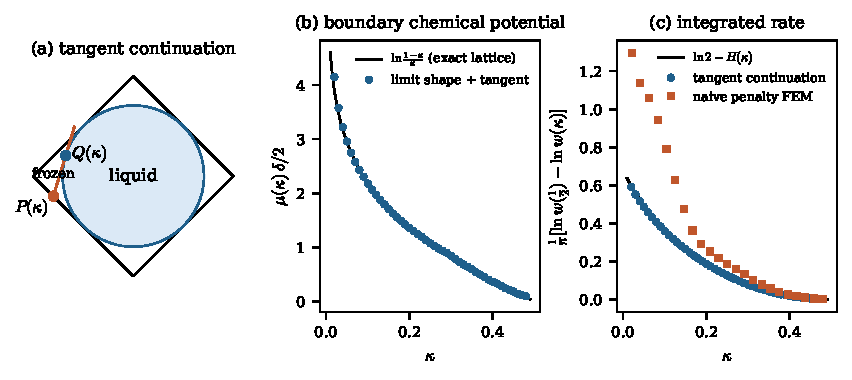
\includegraphics[width=\textwidth]{figs/fig7_aztec_mu.pdf}
\caption{Boundary chemical potential of the Aztec diamond. (a) The dual variables are constant along tangent lines to the arctic circle, so $\mu$ at the edge point $P(\kappa)$ is set by the tangency point $Q(\kappa)$. (b) $\mu(\kappa)$ from the limit shape with tangent continuation (symbols, extracted from a finite-element limit shape) against the exact lattice value $\ln[(1-\kappa)/\kappa]$ (line). (c) Integrated rate: exact continuum result (line), tangent continuation (circles) and the naive penalty-regularized linear response (squares), which is biased by a factor of about $1.45$.}
\label{fig:azmu}
\end{figure*}

\subsection{A mixed domain}
As a test with no free parameter we consider a ``house'': an $N\times N$ square whose two upper corners are cut by staircases of opposite colours (size $k$). The staircases balance the colours, and removing a1 creates one defect. Exact integer computations up to $N=128$ show that the defect leaves a1, the Coulomb attractor, and is trapped on the staircase of the same colour with weight $w\simeq e^{RN}N^{-1}$. The exact rates are $R=0.213$ for $k=N/2$ and $R=0.255$ for $k=N/4$. We computed the limit shape by finite elements. We evaluated $\mu$ directly where the boundary is liquid-adjacent and by tangent continuation where it is frozen, and integrated Eq.~\eqref{eq:mu} along $\Gamma$. This predicts $R=0.204$--$0.217$ and $0.259$--$0.271$ (range over meshes $N=48$--$96$), with the optimum at $x/N=0.07$--$0.09$ (exact: $0.08$--$0.09$), as shown in Fig.~\ref{fig:house}. Most of the gain comes not from the staircase but from the straight left edge, because the staircases tilt the adjacent liquid. The optimum sits where $\mu$ changes sign on the staircase.

\begin{figure*}[t]
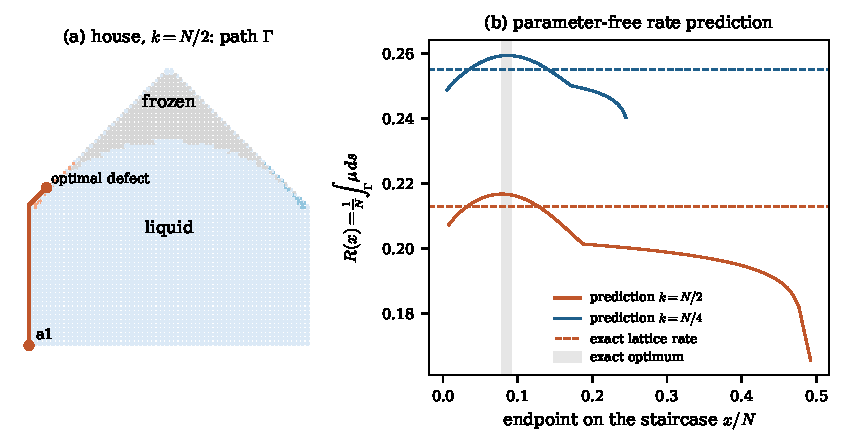
\includegraphics[width=\textwidth]{figs/fig8_house.pdf}
\caption{House-shaped domain. (a) Limit shape ($k=N/2$): liquid (blue) and frozen phases, together with the defect path $\Gamma$ from the removed corner a1 along the straight edge to the optimal point on the staircase. (b) Predicted rate $R(x)=N^{-1}\int_\Gamma\mu\,\dd s$ versus the endpoint $x/N$ for $k=N/2$ and $N/4$ (solid), compared with the exact lattice rates (dashed) and the exact optimal position (grey band).}
\label{fig:house}
\end{figure*}

\subsection{Beyond linear response: layer cost and competing channels}
Confronting Eq.~\eqref{eq:mu} with the exact Aztec laws Eqs.~\eqref{eq:thmC}--\eqref{eq:thmE} reveals two further ingredients. They matter whenever $\Gamma$ runs along \emph{frozen} edges. First, the local gradient of $\ln w$ is always given correctly by Eq.~\eqref{eq:muaztec}, but the rate itself is smaller than $\int_\Gamma\mu$ by exactly $\ln2$. Second, for two defects close to a corner the dominant contribution comes from $j<n$ in Eq.~\eqref{eq:thmE}. All three families are described by the single rule
\begin{equation}
\frac1n\ln w=\max_{\tau}\Bigl[\tau\,L\!\Bigl(\frac\kappa\tau,\frac\lambda\tau\Bigr)-\frac1n\,\frac{\partial\ln Z(\Omega_m)}{\partial m}\Big|_{m=\tau n}\Bigr],
\label{eq:rule}
\end{equation}
where $\Omega_{\tau n}$ is the scaled copy of the domain sharing the relevant corner, $L$ is the linear response $\int_\Gamma\mu$ computed in the unit domain, and the second term is the entropy cost of removing one lattice layer. For the Aztec diamond the layer cost is $\tau\ln2$. Only $\tau=1$ is allowed if an endpoint lies on an edge not containing the corner. Equation~\eqref{eq:rule} reproduces Eqs.~\eqref{eq:thmC} (optimum $\tau=\min(2\kappa,1)$), \eqref{eq:thmD} and \eqref{eq:thmE} exactly. At the lattice level, a defect on a frozen staircase forces a zipper of dominoes (Appendix~\ref{app:proofs}). Two zippers meeting at the corner strip one layer off the inner domain, and the turning point of the zippers is $\tau$. When $\Gamma$ lies entirely on liquid-adjacent edges no zipper forms and Eq.~\eqref{eq:rule} reduces to linear response, which is the situation of the house domain above.

\subsection{Independent test: lozenge tilings of hexagons}
To test Eq.~\eqref{eq:rule} away from the data that suggested it, we studied lozenge tilings of a hexagon with side lengths $a$ (bottom), $b$ (right) and $c$. We remove an up-triangle at distance $k$ and a down-triangle at distance $l$ from the bottom-right corner. By the Lindstr\"om--Gessel--Viennot lemma~\cite{Lindstrom1973,GesselViennot1985}, the number of tilings is a $(c+1)\times(c+1)$ determinant of binomial coefficients. The sources are $(-i,i)$ and $(a-k,1)$, and the sinks are $(a-j,b+j)$ and $(a-1,l)$. We verified this formula against Kasteleyn determinants for all dent positions in three hexagons, and it allows exact computation up to $n=240$.

With the corner triangle fixed, the dent position follows $P(X=m)\propto\binom{a-1+m}{m}\binom{c-1+b-m}{b-m}$. Consistency of Eq.~\eqref{eq:rule} then \emph{requires} a layer cost equal to $\max f-f(0)$, where $f$ is the large-deviation function of $X$. For five hexagons this number equals $\partial\ln Z/\partial c$ to three or four digits and differs clearly from $\partial_a\ln Z$ and $\partial_b\ln Z$ (Fig.~\ref{fig:lozenge}b). The removed layer is therefore the one in the defect-free direction. With no further input, Eq.~\eqref{eq:rule} then predicts the pair rates, including channels with $\tau\approx0.24$--$0.76$ where linear response alone fails completely (e.g.\ $0.003$ instead of $0.139$). The agreement with the exact values is within $0.1$--$0.5\%$ for nine cases in three hexagons (Table~\ref{tab:lozenge}). Along the diagonal $\kappa=\lambda$ it holds at twenty further points in two hexagons, with deviations below $0.3\%$ (Fig.~\ref{fig:lozenge}a).

\begin{figure*}[t]
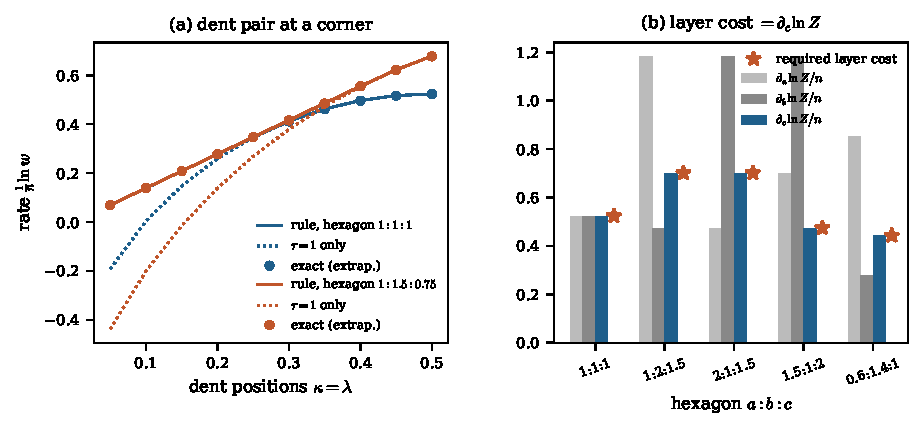
\includegraphics[width=\textwidth]{figs/fig9_lozenge.pdf}
\caption{Independent test on lozenge tilings. (a) Rate of a dent pair at distances $\kappa=\lambda$ from a corner, for two hexagons: exact values extrapolated from $n=60,120,240$ (symbols), the rule Eq.~\eqref{eq:rule} (solid) and linear response alone, $\tau=1$ (dotted). (b) The layer cost required for consistency (stars) coincides with $\partial_c\ln Z/n$, the derivative with respect to the side length in the defect-free direction, and not with $\partial_a$ or $\partial_b$.}
\label{fig:lozenge}
\end{figure*}

\begin{table}[t]
\caption{Pair rates $\frac1n\ln w$ for dents at distances $(\kappa,\lambda)$ from a corner of the hexagon $H(a{:}b{:}c)$. Columns: linear response only ($\tau=1$), the rule Eq.~\eqref{eq:rule} with its optimal $\tau$, and exact values extrapolated from $n=40$--$240$ with $a+b\ln n/n+c/n$.}
\label{tab:lozenge}
\begin{ruledtabular}
\begin{tabular}{lcccc}
$a{:}b{:}c$ & $(\kappa,\lambda)$ & $\tau=1$ & rule ($\tau^*$) & exact \\
\hline
$1{:}1{:}1$ & $(0.1,0.1)$ & $0.003$ & $0.1387$ ($0.37$) & $0.1386$\\
$1{:}1{:}1$ & $(0.2,0.2)$ & $0.259$ & $0.2774$ ($0.75$) & $0.2766$\\
$1{:}1{:}1$ & $(0.1,0.3)$ & $0.208$ & $0.2251$ ($0.76$) & $0.2244$\\
$1{:}1{:}1$ & $(0.3,0.3)$ & $0.412$ & $0.4124$ ($1$) & $0.4111$\\
$1{:}1.5{:}0.75$ & $(0.1,0.1)$ & $-0.201$ & $0.1387$ ($0.24$) & $0.1382$\\
$1{:}1.5{:}0.75$ & $(0.15,0.3)$ & $0.172$ & $0.2866$ ($0.52$) & $0.2865$\\
$1{:}1.5{:}0.75$ & $(0.3,0.6)$ & $0.573$ & $0.5728$ ($1$) & $0.5718$\\
$1.4{:}0.8{:}1$ & $(0.3,0.15)$ & $0.268$ & $0.2866$ ($0.75$) & $0.2850$\\
$1.4{:}0.8{:}1$ & $(0.6,0.4)$ & $0.554$ & $0.5544$ ($1$) & $0.5534$\\
\end{tabular}
\end{ruledtabular}
\end{table}

%=====================================================================
\section{Control: no charge, no long-range boundary effect}
\label{sec:triangle}
%=====================================================================
On the non-bipartite triangular lattice there is no height field. Monomers then carry only a $\mathbb Z_2$ label and no U(1) charge~\cite{FendleyMoessnerSondhi2002}. Pfaffian computations on rhombi with $60^\circ$ and $120^\circ$ corners show a boundary layer of one or two cells, beyond which the defect distribution is flat. The corner-to-centre ratio saturates instead of scaling (Fig.~\ref{fig:tri}). This contrasts with the $N^{-1/4}$ law of the odd square board and confirms that the long-range corner physics requires the emergent charge.

\begin{figure*}[t]
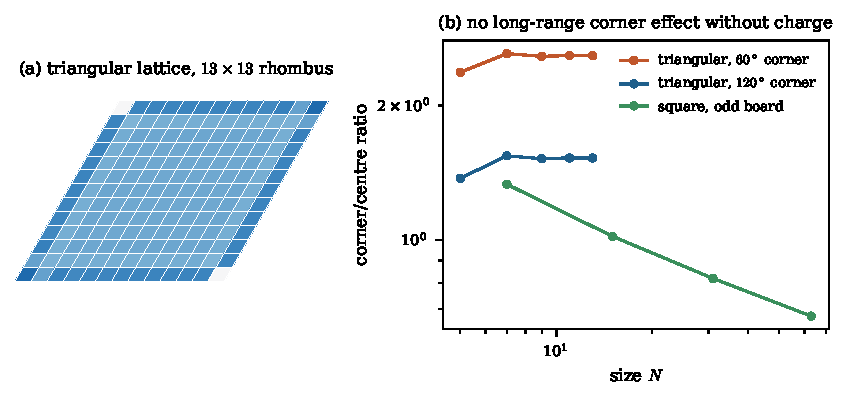
\includegraphics[width=0.85\textwidth]{figs/fig10_triangular.pdf}
\caption{Control on the triangular lattice. (a) Monomer probability on a $13\times13$ rhombus (normalized to uniform). (b) Corner-to-centre ratio versus size: saturation for the triangular lattice ($60^\circ$, $120^\circ$) against the power law $N^{-1/4}$ of the square lattice.}
\label{fig:tri}
\end{figure*}

%=====================================================================
\section{Discussion and conclusions}
\label{sec:conclusion}
%=====================================================================

Forced defects in dimer coverings are pushed around by forces that are entirely entropic. Nevertheless they obey an electrostatics with fractional corner charges and same-sign images. Its origin is the Gauss law imposed by close packing, together with the Gaussian fluctuations of the height field. Entropy only sets the stiffness (the dielectric constant). The resulting picture is quantitative. A single formula, Eq.~\eqref{eq:density}, with charges fixed by boundary height jumps, describes all rectangular geometries without parameters. The corresponding lattice amplitudes factorize into a universal bulk monomer normalization, which is transcendental and contains $G(\tfrac12)^2$, and elementary boundary and corner normalizations. All string determinants reduce to a single scalar Fisher--Hartwig symbol.

The emergent-electrostatics picture breaks down where the boundary freezes the dimer sea. The breakdown is controlled by the boundary chemical potential: the entropy cost of shifting the boundary height, evaluated on the limit shape and continued along tangent lines into the frozen regions. With this one ingredient the Aztec-diamond law is reproduced identically and trapping rates in mixed domains are predicted to a few per cent. Along frozen edges a geometric layer cost and a competition between nested channels must be added. The resulting rule, Eq.~\eqref{eq:rule}, which we inferred from the Aztec diamond, predicts exact lozenge-tiling data to within half a per cent.

The same questions arise wherever constrained degrees of freedom produce emergent Coulomb physics with boundaries. Examples are monopoles in finite spin-ice samples and nanostructures, defects in artificial spin ice, where edge and corner populations can be imaged by magnetic force microscopy~\cite{Wang2006,Ladak2010}, dimer adsorbates and molecular monolayers on terraces, and constrained colloidal systems. Our results suggest that corners should act as fractional charges and edges as same-sign mirrors, as long as the constrained phase touching the boundary is critical. Where it is ordered (frozen), defects should instead be trapped exponentially at the points where the ordered and critical regions meet. Interactions between dimers change the stiffness $g$~\cite{Alet2005}, so all exponents in Eq.~\eqref{eq:gamma} should scale with $g$. This offers an experimental handle on the coupling constant.

Several questions remain open. Among them are a proof of the corner-charge density formula for general domains, which is likely accessible through piecewise-Temperleyan and monodromy methods~\cite{Russkikh2018,Dubedat2015}, and the Toeplitz+Hankel asymptotics that would prove the half-plane and quadrant amplitudes. Others are a first-principles justification of the tangent continuation and of the layer rule in general domains, which appears to be related to the tangent method of Colomo and Sportiello~\cite{ColomoSportiello2016}, and the behaviour of many defects, where screening of the corner charges is expected.

\begin{table}[t]
\caption{Summary of results and their status. ``Proof'': rigorous; ``exact'': exact arithmetic or $\geq10$ digits; ``numerical'': agreement at the per-cent level across sizes; ``known'': previously established in the cited work.}
\label{tab:summary}
\begin{ruledtabular}
\begin{tabular}{p{4.6cm}p{3.0cm}}
Result & Status\\
\hline
Corner charge $q_c=-J_c/4$ & proof; cf.~\cite{Allegra2015}\\
Density formula \eqref{eq:density}, exponent \eqref{eq:gamma} & numerical (1--3\%)\\
Quadrant boundary law \eqref{eq:thmA} & proof\\
Scalar-symbol reductions \eqref{eq:reductions} & proof\\
Bulk amplitude $\pi2^{-3/4}G(\frac12)^4$ & proof (axis); known (diagonal)~\cite{Hartwig1966}\\
Half-plane, quadrant amplitudes & exact (18 digits)\\
Aztec laws \eqref{eq:thmC}--\eqref{eq:thmE} & known~\cite{ChhitaYoung2014}; new elementary proofs of \eqref{eq:thmC}, \eqref{eq:thmD}\\
$\mu$ of the Aztec diamond, Eq.~\eqref{eq:muaztec} & exact identity (given tangent continuation)\\
House trapping rates & numerical (5\%)\\
Layer rule \eqref{eq:rule} & conjecture; exact for Aztec, 0.5\% for lozenges\\
Triangular control & numerical\\
\end{tabular}
\end{ruledtabular}
\end{table}

\begin{acknowledgments}
The author thanks the developers of FLINT and Arb, whose exact and certified arithmetic made the large-scale computations possible.
\end{acknowledgments}

\appendix
%=====================================================================
\section{Elementary proofs for the Aztec diamond}
\label{app:proofs}
%=====================================================================
\emph{Boundary switch.} Each white cell $\mathrm{SW}_k$ on the south-west edge has only two neighbours, $b_{k-1}$ and $b_k$, on the adjacent diagonal. If $\mathrm{SW}_k$ is matched to $b_k$, then $\mathrm{SW}_{k+1}$ must also be matched to $b_{k+1}$. The edge therefore consists of $m$ dominoes of one orientation followed by $n-m$ of the other, and the switch position $m$ is unique.

\emph{Sliding bijection.} If the tip $b_0$ is removed, the cells $\mathrm{SW}_1,\dots,\mathrm{SW}_{k-1}$ are forced. Sliding the dominoes $\mathrm{SW}_i$--$b_{i-1}$ to $\mathrm{SW}_i$--$b_i$ for $i<k$ gives a bijection between tilings of $\AD_n\setminus\{t,\mathrm{SW}_k\}$ and tilings of $\AD_n$ with switch $m\ge k$.

\emph{Switch distribution.} Let $I$ be $\AD_n$ minus the two opposite boundary double layers. Removing a corner cell $c$ of $I$ forces a zipper of $n-2$ dominoes, and what remains is a translate of $\AD_{n-1}$ minus its boundary layer. Kuo's graphical condensation~\cite{Kuo2004}, applied to $G=I\cup\{b_m,e_t\}$ with four boundary vertices of alternating colour, together with the switch of the opposite layer, gives $T_n(m)=2^{n-1}[T_{n-1}(m)+T_{n-1}(m-1)]$. Hence $T_n(m)=\binom nm2^{n(n-1)/2}$, which proves Eq.~\eqref{eq:thmC}.

\emph{Opposite edge.} By $180^\circ$ rotation, removing the east tip forces the whole north-east double layer. The south-west switch then leaves exactly two free cells $b_s,b_{s'}$ with $s<j\le s'$. Kuo's identity with two same-colour pairs gives
$Z(I\cup\{b_s,b_{s'}\})=2^{(n-1)(n-2)/2}\binom ns\binom n{s'}\frac{s'-s}{n}$,
and the binomial identity $\sum_{s<j\le s'}\binom ns\binom n{s'}(s'-s)=n2^{n-1}\binom{n-1}{j-1}$ yields Eq.~\eqref{eq:thmD}.

%=====================================================================
\section{Numerical details}
%=====================================================================
Coulomb-gas predictions for rectangles use the Jacobi map $f(u)=\mathrm{sn}(u,k)$, with the modulus fixed by the aspect ratio. Limit shapes were computed by minimizing the Cohn--Kenyon--Propp functional with the domino entropy written in terms of the Lobachevsky function. We used a finite-element mesh with four triangles per cell, which avoids locking at the slope constraint, and penalty continuation. On the Aztec diamond this reproduces the entropy to $0.02\%$ and the frozen area fraction $1-\pi/4$. Rates were extrapolated using $a+b\ln n/n+c/n$.

%=====================================================================
\begin{thebibliography}{99}
\bibitem{Kasteleyn1961} P. W. Kasteleyn, Physica \textbf{27}, 1209 (1961).
\bibitem{TemperleyFisher1961} H. N. V. Temperley and M. E. Fisher, Philos. Mag. \textbf{6}, 1061 (1961).
\bibitem{FisherStephenson1963} M. E. Fisher and J. Stephenson, Phys. Rev. \textbf{132}, 1411 (1963).
\bibitem{Hartwig1966} R. E. Hartwig, J. Math. Phys. \textbf{7}, 286 (1966).
\bibitem{Kenyon2000} R. Kenyon, Ann. Probab. \textbf{28}, 759 (2000).
\bibitem{Kenyon2001} R. Kenyon, Ann. Probab. \textbf{29}, 1128 (2001).
\bibitem{Nienhuis1984} B. Nienhuis, J. Stat. Phys. \textbf{34}, 731 (1984).
\bibitem{Henley2010} C. L. Henley, Annu. Rev. Condens. Matter Phys. \textbf{1}, 179 (2010).
\bibitem{Huse2003} D. A. Huse, W. Krauth, R. Moessner, and S. L. Sondhi, Phys. Rev. Lett. \textbf{91}, 167004 (2003).
\bibitem{Castelnovo2008} C. Castelnovo, R. Moessner, and S. L. Sondhi, Nature \textbf{451}, 42 (2008).
\bibitem{Wang2006} R. F. Wang \emph{et al.}, Nature \textbf{439}, 303 (2006).
\bibitem{Ladak2010} S. Ladak, D. E. Read, G. K. Perkins, L. F. Cohen, and W. R. Branford, Nat. Phys. \textbf{6}, 359 (2010).
\bibitem{FendleyMoessnerSondhi2002} P. Fendley, R. Moessner, and S. L. Sondhi, Phys. Rev. B \textbf{66}, 214513 (2002).
\bibitem{PriezzhevRuelle2008} V. B. Priezzhev and P. Ruelle, Phys. Rev. E \textbf{77}, 061126 (2008).
\bibitem{Ciucu2010} M. Ciucu, Trans. Amer. Math. Soc. \textbf{362}, 4921 (2010).
\bibitem{CiucuKrattenthaler2011} M. Ciucu and C. Krattenthaler, Commun. Math. Phys. \textbf{302}, 253 (2011).
\bibitem{Allegra2015} N. Allegra, Nucl. Phys. B \textbf{894}, 685 (2015).
\bibitem{JockuschProppShor1998} W. Jockusch, J. Propp, and P. Shor, arXiv:math/9801068 (1998).
\bibitem{CohnKenyonPropp2001} H. Cohn, R. Kenyon, and J. Propp, J. Amer. Math. Soc. \textbf{14}, 297 (2001).
\bibitem{KenyonOkounkov2007} R. Kenyon and A. Okounkov, Acta Math. \textbf{199}, 263 (2007).
\bibitem{DeiftItsKrasovsky2011} P. Deift, A. Its, and I. Krasovsky, Ann. Math. \textbf{174}, 1243 (2011).
\bibitem{BasorEhrhardt2017} E. Basor and T. Ehrhardt, Oper. Theory Adv. Appl. \textbf{259} (2017); arXiv:1603.00506.
\bibitem{GharakhlooIts2020} R. Gharakhloo and A. Its, SIGMA \textbf{16}, 100 (2020).
\bibitem{EKLP1992} N. Elkies, G. Kuperberg, M. Larsen, and J. Propp, J. Algebraic Combin. \textbf{1}, 111 (1992); \textbf{1}, 219 (1992).
\bibitem{ChhitaYoung2014} S. Chhita and B. Young, Adv. Math. \textbf{259}, 173 (2014).
\bibitem{CohnElkiesPropp1996} H. Cohn, N. Elkies, and J. Propp, Duke Math. J. \textbf{85}, 117 (1996).
\bibitem{Lindstrom1973} B. Lindstr\"om, Bull. London Math. Soc. \textbf{5}, 85 (1973).
\bibitem{GesselViennot1985} I. Gessel and G. Viennot, Adv. Math. \textbf{58}, 300 (1985).
\bibitem{Kuo2004} E. H. Kuo, Theor. Comput. Sci. \textbf{319}, 29 (2004).
\bibitem{Alet2005} F. Alet, J. L. Jacobsen, G. Misguich, V. Pasquier, F. Mila, and M. Troyer, Phys. Rev. Lett. \textbf{94}, 235702 (2005).
\bibitem{Russkikh2018} M. Russkikh, Probab. Theory Relat. Fields \textbf{171}, 281 (2018).
\bibitem{Dubedat2015} J. Dub\'edat, J. Amer. Math. Soc. \textbf{28}, 1063 (2015).
\bibitem{ColomoSportiello2016} F. Colomo and A. Sportiello, J. Stat. Phys. \textbf{164}, 1488 (2016).
\end{thebibliography}

\end{document}
